\section{AEM}

\paragraph{}
A company that makes a similar product is AEM Electronics.
AEM designs data loggers and dashboards for testing purposed for cars and other vehicles.
These dataloggers connect to their different modules that connnect to various can sensors and breakouts for different types of sensors.
Some of these modules also come with an inertial measurement units (IMU) and global positioning system (GPS) which are useful for understanding the entire vehicle state.

\subsection{AEM Loggers}

\paragraph{}
There are several different AEM loggers available for purcahse.
The two major loggers available for purchase are the AEM CD-5L and the AEM CD-7L.
The CD-5L costs \$1,574.95 without the IMU or GPS and the CD-7L costs \$2,081.95 without the IMU or GPS \cite{AEMSite}.
This cost provides access to data logging features as well as a dashbaord display.
These dashboards can be configured to display different information to a driver or engineer to get a snapshot of the current state of the vehicle.
A computer can be easily connected to these devices to upload different configurations as well as to download the logged files.

\begin{figure}[H]
	\centering
	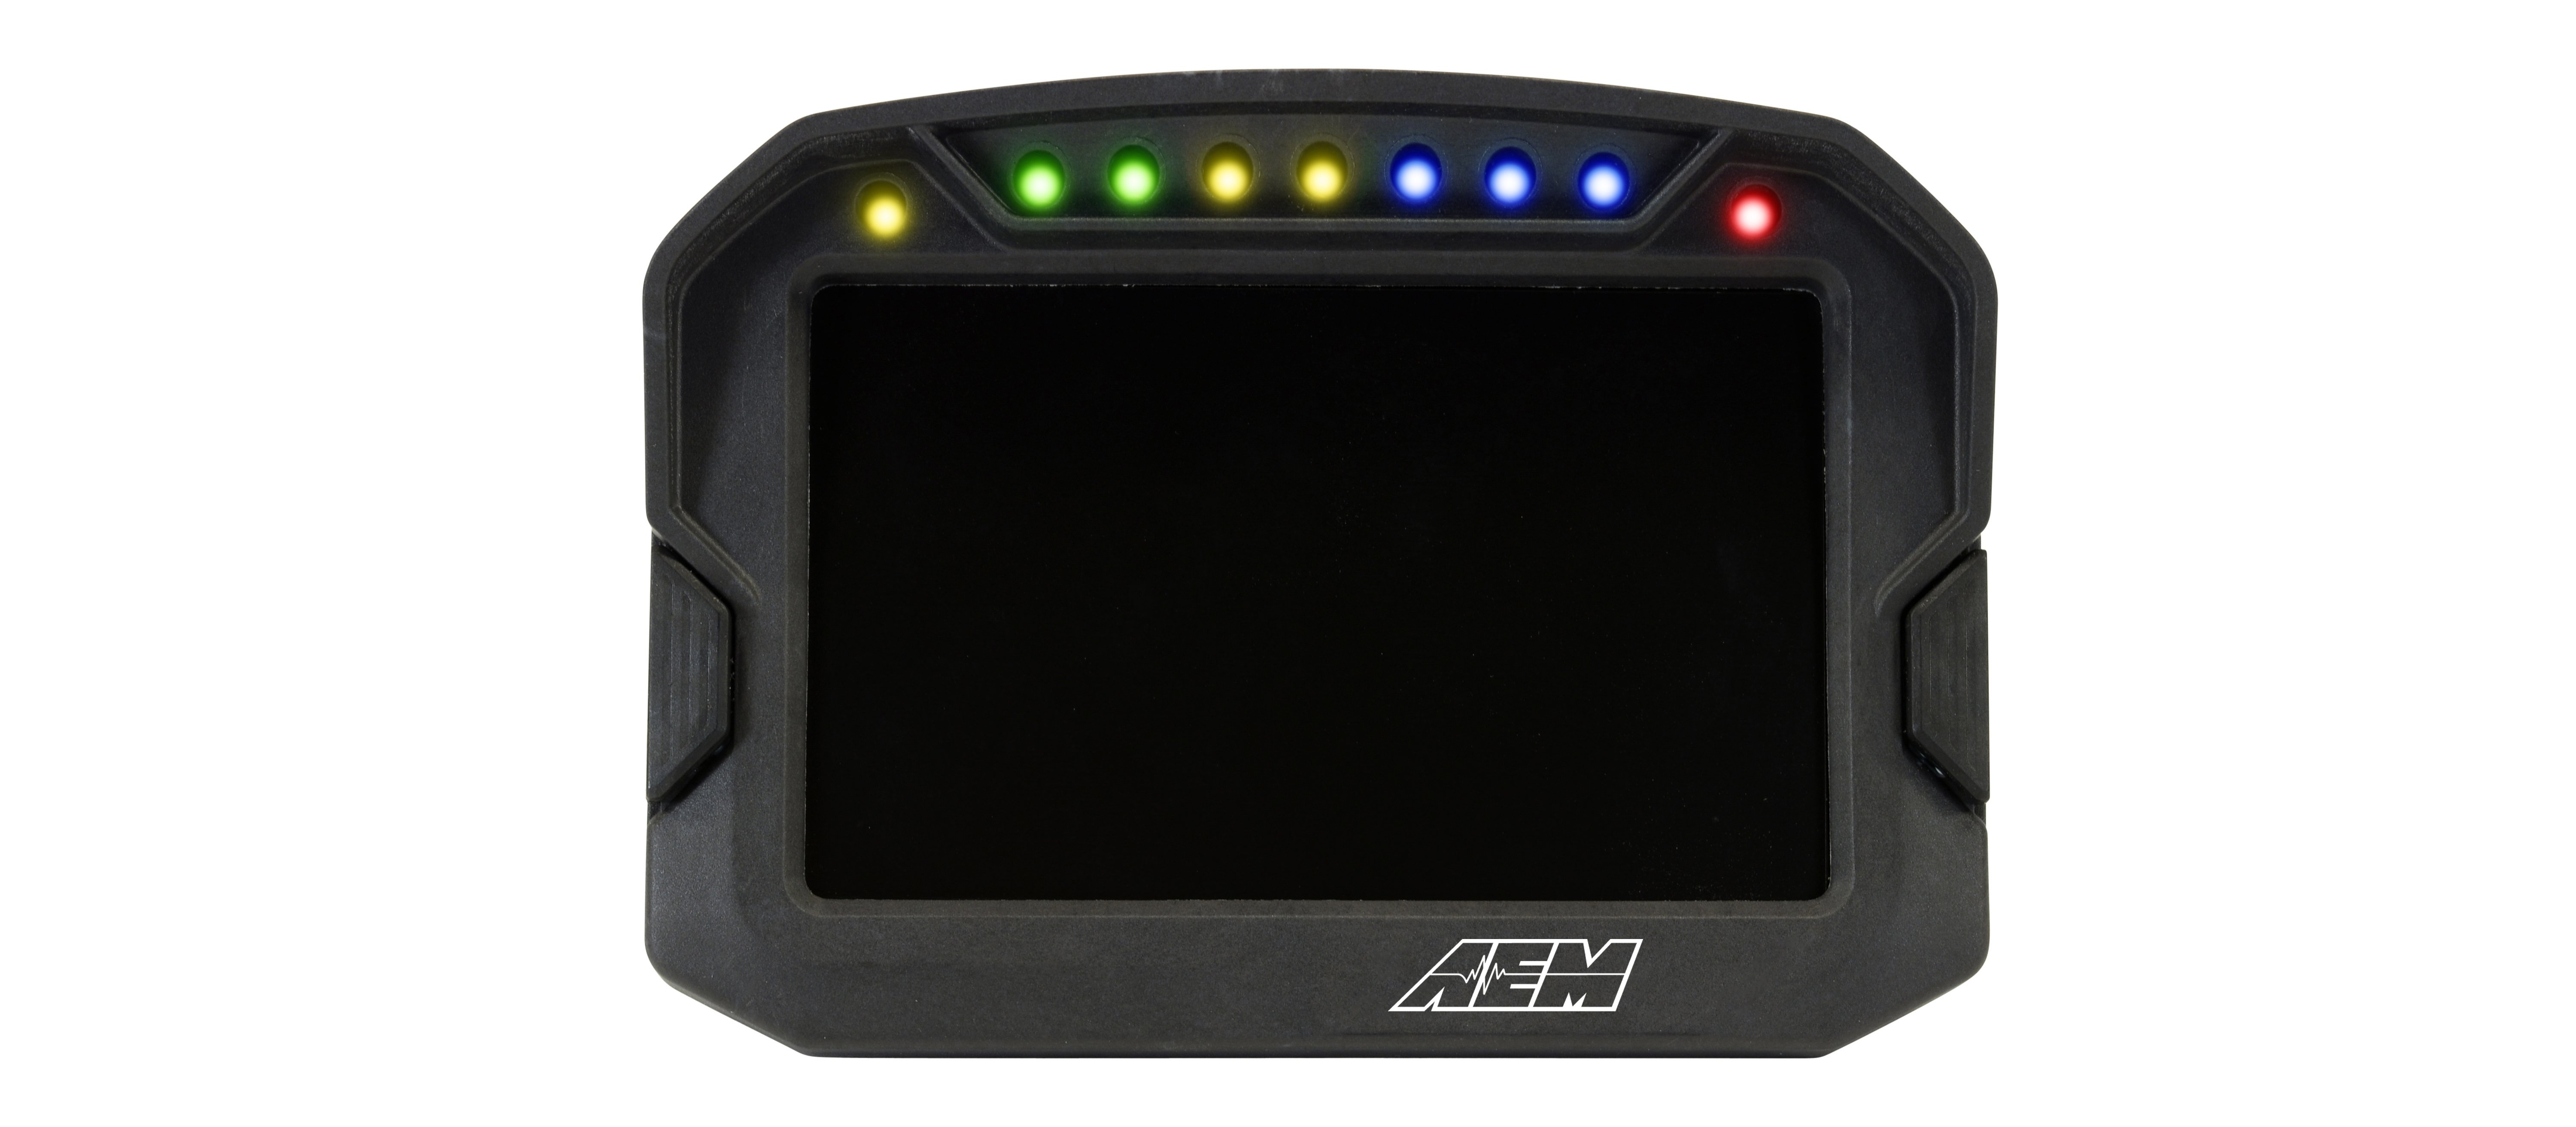
\includegraphics[width=\linewidth]{AEM_CD5.jpg}
	\caption{AEM CD5L Dashboard}
	\label{fig:AEM_CD5}
\end{figure}

\paragraph{}
The loggers log files in a comma seperated file (csv) format for ease of use with tools such as Matlab or Python for visualizing the data.
These files can also be visualized on the dashboard as well to give a quick glimpse at explaining what is happening.

\subsection{AEM Add-Ons}

\paragraph{}
In order to connect more sensors or instrumentation to the AEM loggers, additional add-ons must be purchased and configured.
Some of these add-ons include a CAN module which allows the AEM logger to connect to and interface with a CAN bus and a thermocouple unit for measuring temperature.
These expansion units, before the cost of any sensors, are several hundred dollars on their own.
In order to hook up any sensors, at least one of these expansion units must be purchased.

\begin{figure}[H]
	\centering
	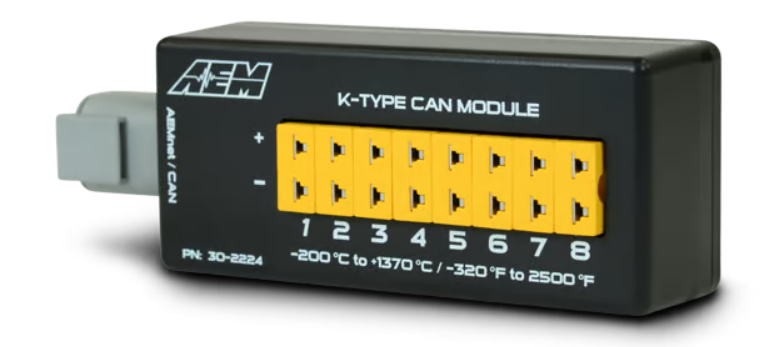
\includegraphics[width=\linewidth]{AEM_THERMO.png}
	\caption{AEM thermocouple expansion unit}
	\label{fig:AEM_THERMO}
\end{figure}

\paragraph{}
AEM also sells some sensors that are simple to integrate into their ecosystem.
These sensors include thermocouples, air and water temperature sensors, and several styles of pressure transducers.
Each of these sensors is somewhat expensive on their own, costing around \$100 per individual sensor.
The AEM loggers can also interface with traditional analog or digital sensors so long as the appropriate add-ons are purchased.

\paragraph{}
In addition to wired sensors, AEM is also compatible with some wireless sensors for things such as tire pressure monitoring systems (TPMS) or fuel sensors.
In order to communicate with these wireless sensors, a wireless module in needed or a logger with wireless capabilities is needed.
AEM utilies a propietary system call X-Wifi to connect to these wireless sensors that is already a part of their CD5 and CD7 loggers.
AEM's sensors that can utilize the X-Wifi capabilities of the logger are priced Similarly to their more traditional wired sensors.

\subsection{DBC Files}

\paragraph{}
In addition to AEM specific sensors, the AEM dataloggers can interface with any custom hardware that is outputting it's data over CAN.
In order to configure the AEM to read data from a CAN bus, including its own CAN capable sensors, a configuration file must be made to tell the logger which value corresponds to which bytes of a specific CAN frame.
A CAN Database file (.dbc) is a standarized file format for configuring which is able to describe what information is contained within a CAN frame.
An example .dbc file can be seen in \cref{lst:ex_dbc} in the appendix.
AEM utilizes this file format for its dataloggers to interface with a CAN network so long as the proper hardware add-ons are purchased.